%-------------------------------------------------------------------------------
\section{Introduction}
%-------------------------------------------------------------------------------
Web application developers today have more incentives than ever to provide better privacy for their
users.
%
Laws like the EU's General Data Protection Regulation (GDPR)~\cite{eu:gdpr} and California's
Consumer Privacy Act (CCPA)~\cite{ca:privacy-act} codify users' right to be forgotten, and restrict
any data retention to anonymized information.
%
Legal consequences and the reputational damage associated with data breaches~\cite{breach:amazon,
breach:twitter, breach:fb, breach:marriott, breach:quora} make it good practice to minimize the user
data retained.
%

%
Although many developers are well-intentioned, today they must manually implement \emph{privacy
transformations}---such as user account deletion or data minimization---which burdens
them with complexity and results in ad-hoc solutions. %(\S\ref{sec:survey}).
%\lyt{add other examples of transformations? e.g., anonymization when exporting data, for data
%minimization, to support user-chosen privacy settings? we do only really talk about user account
%deletion in webapps today, though}
%
%
To write a privacy transformation, developers must carefully map the high-level privacy policy to
operations that delete or rewrite data objects, while ensuring that the application preserves
utility for other users, retains legally-mandated anonymized data, and avoids violating application
invariants.
%
For example, deleting a user's account should not unexpectedly grant broad access to
previously-private content by deleting objects that restrict access, nor should it make
non-sensitive shared content disappear.
%
Developers must also consider indirectly identifying correlations between data objects: for example,
anonymized public running routes can identify the user's hometown and even the
user~\cite{strava:heatmap}, and anonymized order histories in e-commerce sites can reidentify
buyers.

\begin{figure}[t]
    \centering
    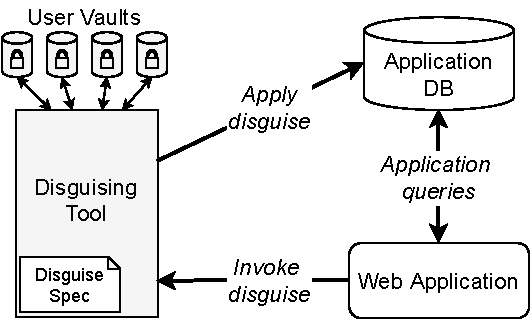
\includegraphics[width=0.35\textwidth]{img/disguise_tool}

    \caption{A data disguising tool sits alongside the application code and database.}
    \label{fig:tool}
\end{figure}


\iffalse
To get privacy transformations right, developers must carefully map the high-level privacy
policy to operations that delete or rewrite data objects, while ensuring that the application preserves
utility for other users, retains legally-mandated anonymized data, and avoids violating
application invariants.
%
For example, deleting a user's account should not unexpectedly grant broad
access to previously-private content by deleting objects that restrict access,
nor should it make non-sensitive shared content disappear.
%
Privacy transformation designers must correctly handle identifying data, as well as indirectly identifying
correlations between data objects.
For example, anonymized public running routes can identify the user's hometown and be
reassociated with the user~\cite{strava:heatmap},
%anonymized posts on Reddit correlated with a subreddit with very few subscribers can be
%associated back to a single user;
% papers' affiliation and reviewer conflicts in HotCRP can reidentify the author;
and anonymized order histories in e-commerce sites can reidentify buyers.
\fi

%
The burden of implementing privacy transformations grows with the underlying privacy policy's
complexity.
%
Although simplicity has advantages, more nuanced privacy policies are important and useful.
%
Such policies can help protect users against data correlation attacks; they can give more
control to individuals by allowing them to choose their own, fine-grained privacy semantics; and
they may enable new privacy modes such as data that gradually ``decays'' to become less identifiable over time.
%
Likewise, reversible privacy transformations might strike a sweet
spot---allowing users to remove identifiable information on demand,
but accommodating service providers' interest to make it easy for users to return---but
add significant implementation burden.
%

%
With more nuanced and reversible privacy transformations, developers face an even greater challenge:
they must reason about how these privacy transformations compose. For example, an application may
automatically decay data over time, but must still correctly remove a user's data when they delete
their account, even if this data has been anonymized.
Ensuring that one privacy transformation does not affect the privacy properties
achieved by future transformations, even if they both transform the same data, is a non-trivial task.
%

%
We propose \emph{data disguising}, a new framework
for systematically specifying, implementing, and reasoning about  privacy transformations.
%
In this framework, developers specify transformations required in privacy policies as
high-level \emph{data disguises} over existing application data types and associations.
%
Applying a disguise transforms the state of application data in privacy-preserving ways (\eg
deleting users' identifiers, or decorrelating identifying object relationships) while preserving
application invariants and utility.
%
Disguises do not guarantee strict privacy---a disguise's content might still expose user
information or correlated data if not redacted by the policy---but flexible disguising,
rather than universal deletion, is what real applications require.
%
%Disguises consist of transformations performed on the high-level object graph embedded in
%database-based applications (encoded by \eg foreign key relationships in relational
%databases)~\cite{orms}.

A data disguising tool takes a disguise and its target, and automatically applies the appropriate
transformations to application data to achieve the disguised state, handling
disguise composition and disguise interdependencies. Developers can
thus reason at a high level about each disguise in isolation, reducing the developer burden.
%

Our proof-of-concept, \sys, demonstrates the potential of such a tool.
%
\sys proxies relational database operations and exposes APIs to invoke privacy transformations.
%

\section{Privacy Transformations}
\label{sec:survey}

\subsection{Privacy Transformations In Practice Today}
%
We surveyed widely-used web applications to understand the privacy
transformations they apply.
%
The main privacy transformation these applications support is account deletion,
a transformation that \eg the GDPR~\cite[Art.\ 17]{eu:gdpr} mandates.
%
%~\cite{facebook:privacy, twitter:privacy, hotcrp:privacy, reddit:privacy,
%github:privacy, hackernews:privacy, strava:privacy, linkedin:privacy, stackoverflow:privacy,
%wikipedia:privacy, amazon:privacy, prestashop:privacy, spotify:privacy, lobsters:privacy}:


%\paragraph{Treatment of user contributions.}
%
On account removal, all applications surveyed delete some user profile
information (\eg passwords) from underlying databases, but all applications
also retain some information for legal or necessary business purposes
(\eg Spotify fraud detection~\cite{spotify:privacy}, PrestaShop/Amazon
orders~\cite{amazon:privacy, prestashop:privacy}).
%
The treatment of other user contributions varies.
%
Some services keep most contributions publicly and indefinitely available (\eg StackOverflow
answers~\cite{stackoverflow:privacy}, shared Strava routes~\cite{strava:privacy}), sometimes
associated with the original user name (\eg Wikipedia edit history~\cite{wikipedia:privacy}), even
if a user deletes their account.
%
Social networking platforms delete some of a user's contributions (\eg
posts), but keep others unanonymized and visible to their recipients (\eg
Facebook/Twitter private messages~\cite{facebook:privacy, twitter:privacy},
LinkedIn updates~\cite{linkedin:privacy}).
%
Other platforms with mostly public content keep user contributions visible to the intended
audience, but anonymize them by reattributing the contribution to a placeholder user
(\eg GitHub's ``@ghost''~\cite{github:privacy}, Reddit and Lobsters'
``[deleted]''~\cite{reddit:privacy, lobsters:privacy}).
%
%    \item Keep certain user contributions unanonymized and visible to its intended audience (\eg
%        HotCRP, Lobsters, Wikipedia, HackerNews~\cite{hotcrp:privacy, lobsters:privacy,
%        hackernews:privacy, wikipedia:privacy}).
%    \item Delete user contributions on user profile or feed (\eg Facebook,
%        Twitter~\cite{facebook:privacy, twitter:privacy}).
%\end{itemize}
%

In the open-source applications surveyed, developers implement privacy transformations
via ad-hoc database operations, and only trigger them on explicit, user-initiated account
deletion.
%
Most developers appear to pay little attention to identifying correlations
within the remaining data.
%


\subsection{Desirable Privacy Transformations Missing Today}

\paragraph{Nuanced policies.}
%
Users and application developers can both benefit from more nuanced privacy policies.
%
For example, a confidential paper review system like HotCRP~\cite{hotcrp} must keep a
user's contributions
(papers, reviews) after they delete their account to preserve utility for others, but could
associate each review with a different placeholder to avoid revealing the deleted reviewer's
identity.
%
%Likewise, contributions with a shared property (\eg Reddit posts with a common tag)
%might be removed entirely to avoid inference attacks, or retained and decorrelated from the
%property (\ie keeping the user's Reddit posts, but removing their tags).
%\eddie{Would like more explanation of that}
In some cases, a policy could preserve utility while reducing the efficacy of later inference
attacks by changing posts, such as by modifying their metadata (\eg tags, posting times).
%
Some transformations should be performed only on sensitive metadata:
%Similar policies could apply \emph{only if} the property was created by the user (\eg keeping
%the user's Reddit posts, but removing any user-created tags),
a tag like “\#cat” is likely insensitive and useful to preserve, whereas one naming a person is not.
%
%(\eg remove the user's posts on Reddit with tag $t$ if these posts comprise more than 10\%
%of all posts with tag $t$).
%
Individual users may even specify different preferences for their data.
%
%% A privacy transformation framework is necessary to turn these preferences into concrete
%% operations without undue developer burden.
%

\paragraph{Data decay.}
%
Applications could go beyond simple account deletion and support a data expiration policy that
anonymizes a user's contributions after the user has been inactive for a period of time,
possibly restoring the user's profile and contributions if the user ever logs back in.
%
Or the application could gradually ``decay'' sensitive data by applying several privacy
transformations that incrementally remove identifiable information over time.
%from it as it ages.
%
%% This requires periodic, automated privacy transformations.

\paragraph{Reversibility.}
%
Many applications might wish to employ \emph{reversible} transformations to, for example, support
account reactivation instead of permanent and irrevocable account deletion.
%
After all, if services must allow users to remove their data on request, it is in the operator's
interest as well as the user's to make it easy for a user to change their mind and return, bringing their data along.
%
%An advanced reversible transformation might record all data transformed, and push an encrypted
%archive to third-party cloud storage.
%
%If the user wishes to return, they supply the archive to reverse the transformation.
%
%To ensure access even if the user loses their key, the transformation might secret-share
%the encryption key~\cite{secretsharing} among the user, the service, and a trusted third party (\eg
%the ACLU or EFF).
%

\subsection{The Future of Privacy Transformations}
%
\ms{This doesn't fit well currently.}
\lyt{Took a shot a rewording/reorganizing...}
%
Privacy transformations and their potential properties allow them to act as powerful mechanisms for
privacy. This argues for a systematic treatment of privacy transformations that makes them a
first-class citizen in application design.
%
In particular, we imagine that developers declaratively specify the above and other
transformation policies like they specify a storage structure (\eg a relational schema) today.
%
This also allows for new policies and use cases that benefit both end-users and service operators.
%
%% Our \emph{data disguising} approach supports these new policies and concepts,
%% which are missing from today's applications but easily described via disguises.
%
